\newpage
\section{Auswertung}
Im folgenden Kapitel werden die aufgenommenen Messwerte ausgewertet und die Ergebnisse 
diskutiert.\\
\textit{Hinweis} beim Aufzeichnen der Messwerte ist ab dem invertierenden Integrator
ein unbekannter Fehler im Experiment aufgetreten. Dieser ist dafür verantwortlich, dass
unsere Messwerte ab diesem Zeitpunkt unbrauchbar geworden sind.
Damit dennoch die wesentlichen Zusammenhänge und Ziele des Experiments gezeigt werden können,
sind Messwerte von zwei unterschiedlichen Gruppen für die weitere Auswertung herangezogen worden
\cite{schmitt}, \cite{signal}, \cite{int_data}, \cite{int_picture}.
Die Benutzung sowie die Quellen der Messwerte
ist in diesem Abschnitt an unterschiedlichen Stellen kenntlich gemacht.

\subsection{Der invertierende Verstärker / Linearverstärker}
\subsubsection{Untersuchung der Verstärkung}
Im ersten Teil des Versuches wird das frequenzabhängige Verhalten der Verstärkung untersucht.
Hierzu wird die Ausgangsspannung in Abhängigkeit der Frequenz über mehrere Dekaden gemessen. 
Anschließend wird die Verstärkung sowie die Frequenz logarithmiert und in einem Plot aufgetragen.
Es werden insgesamt drei unterschiedliche Verstärkungen untersucht.
Die Plots sind sind in \autoref{fig:Linearverstaerker} dargestellt.
Per linearer Regression
\begin{equation}
    %f(x) = mx+b,
    V(f) = m f + b,
    \label{eq:linReg}
\end{equation}
lassen sich die Verstärkung, die Grenzfrequenz und das Bandbreitenprodukt bestimmen.
Hierbei steht $V(f)$ für die Verstärkung, $f$ für die Frequenz, $m$ für die Steigung
und $b$ für den Schnittpunkt der Geradengleichung bei $f = 0$.

Die Fitparameter der drei unterschiedlichen Verstärkungen sind in 
\autoref{tab:fitparams_100},\autoref{tab:fitparams_10} und \autoref{tab:fitparams_1000}
dargestellt.
Hierbei steht die erste Zeile jeweils für die Fitparameter des Plateaus und 
die zweite Zeile für die Steigung des Abfalls.
\input{build/fitparams_100.tex}
\input{build/fitparams_10.tex}
\input{build/fitparams_1000.tex}
\FloatBarrier

Damit die lineare Regression gelingt, werden die Frequenzen und die Ausgangspannung logarithmiert in die
lineare Regression \autoref{eq:linReg} eingesetzt.
Im Plot schwarz markierte Messwerte werden als Ausreißer betrachtet 
und fließen nicht in die Berechnungen ein.
Die errechneten Parameter sind in \autoref{tab:params} dargestellt.
Hierbei ist $V_\text{theo}$ die theoretische Verstärkung, berechnet anhand des gewählten 
Widerstandsverhältnisses, $V_\text{b}$ die gemessene Verstärkung, $f_\text{gr}$ die 
gemessene Grenzfrequenz und $GBP$ das aus den Messwerten 
(vgl. Anhang \ref{sub:Messwerte des Linarverstärkers}) errechnete Bandbreitenprodukt.
\input{build/tabParameter_Linearverstärker.tex}
\FloatBarrier
Werden die gemessenen Plateaus, sprich die gemessenen Verstärkungen, mit den Theorie
Werten verglichen, ergibt sich bei einer Verstärkung von 10 eine Abweichung von ca. 33\% nach oben
und bei einer Verstärkung von 1000 eine Abweichung von 13\% nach oben.

Betrachtet man die unterschiedlichen Graphen so lässt sich erkennen, dass
die jeweiligen Verstärkungen bei niedrigen Frequenzen in guter Näherung konstant
bleiben. Mit steigender Frequenz fällt die Verstärkung im Plot linear ab.
Dies entspricht ganz den Erwartungen der vorangestellten Theorie.
\begin{figure}
    \centering
    \begin{subfigure}[b]{0.45\textwidth}
        \centering
        \includegraphics[width=\textwidth]{build/a.pdf}
        \caption{Linearverstärker bei einer Verstärkung von 100.
        Die eingestellten Widerstandwerte sind $R_1 = \SI{1}{\kilo\ohm}$ und $R_2 = \SI{100}{\kilo\ohm}$. }
        \label{fig:a}
    \end{subfigure}
    \hfill
    \begin{subfigure}[b]{0.45\textwidth}
        \centering
        \includegraphics[width=\textwidth]{build/b.pdf}
        \caption{Linearverstärker bei einer Verstärkung von 10. 
        Die eingestellten Widerstandwerte sind $R_1 = \SI{10}{\kilo\ohm}$ und $R_2 = \SI{100}{\kilo\ohm}$. }
        \label{fig:b}
    \end{subfigure}
    \newline
    \newline    
    \newline    
    \newline    
    \begin{subfigure}[b]{0.45\textwidth}
        \centering
        \includegraphics[width=\textwidth]{build/c.pdf}
        \caption{Linearverstärker bei einer Verstärkung von 1000. 
        Die eingestellten Widerstandwerte sind $R_1 = \SI{100}{\ohm}$ und $R_2 = \SI{100}{\kilo\ohm}$. }
        \label{fig:c}
    \end{subfigure}
       \caption{Aufgenommene Graphen bei unterschiedlichen Verstärkungsfaktoren. Die zugrunde liegende 
       Schaltung ist die des invertierenden Verstärkers \autoref{fig:InvLinear}.}
       \label{fig:Linearverstaerker}
\end{figure}
\FloatBarrier

\subsubsection{Verhalten der Phasendifferenz bei steigender Frequenz}
Im nächsten Teil des Versuches wird die Phasenverschiebung von Ein- und Ausgangsspannung 
untersucht.
Dazu wird die gemessene Phasendifferenz $\phi$ in Abhängigkeit der logarithmierten Frequenz $f$
aufgetragen.
Die Plots sind in \autoref{fig:phase} dargestellt.

Anhand der Plots ist erkennbar, dass mit steigender Frequenz die Phasendifferenz zwischen 
Ein- und Ausgangsspannung sinkt.
Da es sich bei der verwendeten Schaltung um einen invertierenden Verstärker handelt, beginnt 
der Phasenversatz bei $\SI{180}{\degree}$.

Des Weiteren lässt sich erkennen, dass je höher der Verstärkungsfaktor ist, desto früher
beginnt der Phasenversatz zu sinken. 
Bei der \autoref{fig:phase_1000} wurden insgesamt 3 Messwerte rausgenommen und 
als Ausreißer identifiziert.

Betrachtet man insbesondere die \autoref{fig:phase_10} so ähnelt der Verlauf
des Graphen dem Verlauf eines Tiefpasses.
Bei einem Tiefpass können niedrige Frequenzen passieren, wohingegen hohe Frequenzen
unterdrückt werden.

Anschließend lässt sich bei genauerer Betrachtung
der \autoref{fig:Linearverstaerker} und \autoref{fig:phase}
erkennen, dass die Phasen in \autoref{fig:phase} ungefähr dann beginnen zu sinken wenn die Plateaus 
in \autoref{fig:Linearverstaerker} enden.
In \autoref{fig:phase_10} und \autoref{fig:b} ist dies der Fall bei einer Frequenz von ca. 22kHz.

\begin{figure}
    \centering
    \begin{subfigure}[b]{0.45\textwidth}
        \centering
        \includegraphics[width=\textwidth]{build/Phasenbeziehung_100.pdf}
        \caption{Phasenverschiebung zwischen Ein- und Ausgangsspannung bei einer Verstärkung von 100.
        Der Plot entsteht durch die Schaltung des invertierenden Integrators \autoref{fig:UmkehrInt}.
        Die dazugehörigen Messwerte stammen aus \cite{int_data}.
        }
        \label{fig:phase_100}
    \end{subfigure}
    \hfill
    \begin{subfigure}[b]{0.45\textwidth}
        \centering
        \includegraphics[width=\textwidth]{build/Phasenbeziehung_10.pdf}
        \caption{Phasenverschiebung zwischen Ein- und Ausgangsspannung bei einer Verstärkung von 10.
        Der Plot entsteht durch die Schaltung des invertierenden Integrators \autoref{fig:UmkehrInt}.
        Die dazugehörigen Messwerte stammen aus \cite{int_data}.}
        \label{fig:phase_10}
    \end{subfigure} 
    \newline
    \newline   
    \newline   
    \newline   
    \begin{subfigure}[b]{0.45\textwidth}
        \centering
        \includegraphics[width=\textwidth]{build/Phasenbeziehung_1000.pdf}
        \caption{Phasenverschiebung zwischen Ein- und Ausgangsspannung bei einer Verstärkung von 1000.
        Der Plot entsteht durch die Schaltung des invertierenden Integrators \autoref{fig:UmkehrInt}.
        Die dazugehörigen Messwerte stammen aus \cite{int_data}.}
        \label{fig:phase_1000}
    \end{subfigure}
       \caption{Aufgenommene Phasendifferenz bei unterschiedlichen Verstärkungsfaktoren.}
       \label{fig:phase}
\end{figure}
\clearpage

\subsection{Der invertierende Integrator \cite{int_data}, \cite{int_picture}}
In diesem Abschnitt wird überprüft, ob sich die Ausgangsspannung des Integrators antiproportional 
zur Frequenz verhält.
Dazu wird im Experiment die Ein- und Ausgangsspannung in Abhängigkeit der Frequenz gemessen.

Die Messdaten sind in \autoref{tab:integrator} zu finden. 
Wie bereits im obigen Hinweis erwähnt, handelt es sich bei den ausgewerteten Messwerten
um Fremddaten \cite{int_data}, \cite{int_picture}.

Im nächsten Schritt ist die Ausgangsspannung in Abhängigkeit der Frequenz in einem Plot
mit doppellogarithmischer Skala aufgetragen worden.
Dieser Plot ist in \autoref{fig:integrator} zu sehen.
Anschließend wird mit Hilfe der Regressionsfunktion
\begin{equation*}
    ln(f(x)) =  m\,ln(x) + b
\end{equation*}
der erste Bereich (bis ca. 1000\,Hz) gefittet.
Dadurch ist in \autoref{fig:integrator} der blaue Fit entstanden.

Anhand des blauen Fits ist erkennbar, dass sich die Ausgangsspannung antiproportional zu der Frequenz
verhält.
Dies ist genau was man aus der Theorie nach \autoref{eq:Int_Kosinus} erwartet.

Wird allerdings der weitere Verlauf der Messwerte betrachtet, so fällt auf, dass die 
Ausgangsspannung ab ca. 1000\,Hz wieder zu steigen beginnt. 
Dieser Effekt kann zum jetzigen Zeitpunkt noch nicht erklärt werden.
Im weiteren Verlauf beginnt diese aber wieder zu sinken (roter Fit), was der ursprünglichen 
Erwartung entspricht. 
Die beiden Steigungen der Fits sind nahezu gleich, was dafür spricht, dass der Abfall
auf dem selben Effekt beruht.
\begin{align*}
    m_\text{blau} &=  \SI{-0,87\pm0,05}{\volt\per\hertz},\quad b =\SI{6,51\pm 0,20}{\volt} \\
    m_\text{rot} &=  \SI{-0,82\pm0,05}{\volt\per\hertz},\quad b =\SI{11,01\pm 0,20}{\volt}
\end{align*}
\begin{figure}
    \centering
    \includegraphics[width=0.7\linewidth]{build/integrator.pdf}
    \caption{Ausgangsspannung in Abhängigkeit der Frequenz. Der Plot entsteht durch die Schaltung
    des invertierenden Integrators \autoref{fig:UmkehrInt} mit $R = \SI{10}{\kilo\ohm}$ und
    $C = \SI{100}{\nano\farad}$. Entstanden ist der Plot mit  Hilfe der Messdaten von \cite{int_data}.}
    \label{fig:integrator}
\end{figure}
\FloatBarrier
Vergleicht man die Steigungen mit jener der Theorie
\begin{align*}
    m_\text{theo} =  \SI{-1,00}{\volt\per\hertz},\quad b =\SI{7,02}{\volt}
\end{align*}
ergibt sich eine Abweichung von 13\%.

Mit Hilfe der aufgebauten Integratorschaltung lassen sich verschiedene Eingangssignale 
integrieren. 
Im unserem Experiment werden die Integrationen einer Sinus-, einer Dreiecks- und einer Rechteckspannung 
untersucht.
Die Integrationen sind mit Hilfe eines Oszilloskops aufgezeichnet worden.
Daraus ergeben sich die Bilder in \autoref{fig:int}.
\begin{figure}
    \centering
    \begin{subfigure}[b]{0.45\textwidth}
        \centering
        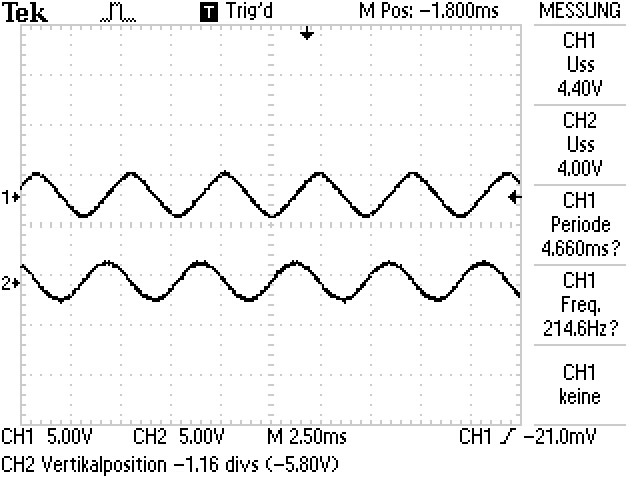
\includegraphics[width=\textwidth]{data_of_others_cuz_ours_suck/int/int_sinus.JPG}
        \caption{Oszillographische Darstellung einer integrierten Sinusspannung.
        Die integrierte Sinusspannung ist auf Channel 2 dargestellt und ist ein Kosinus. \cite{int_picture}}
        \label{fig:int_sin}
    \end{subfigure}
    \hfill
    \begin{subfigure}[b]{0.45\textwidth}
        \centering
        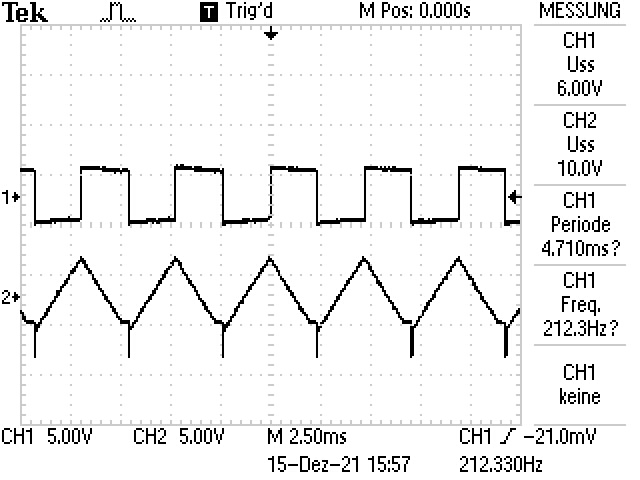
\includegraphics[width=\textwidth]{data_of_others_cuz_ours_suck/int/int_recht.JPG}
        \caption{Oszillographische Darstellung einer integrierten Rechteckspannung.
        Die integrierte Rechteckspannung ist auf Channel 2 dargestellt und ist eine Dreieckspannung.\cite{int_picture}}
        \label{fig:int_recht}
    \end{subfigure}
    \newline
    \newline  
    \newline
    \newline  
    \newline  
    \begin{subfigure}{0.45\textwidth}
        \centering
        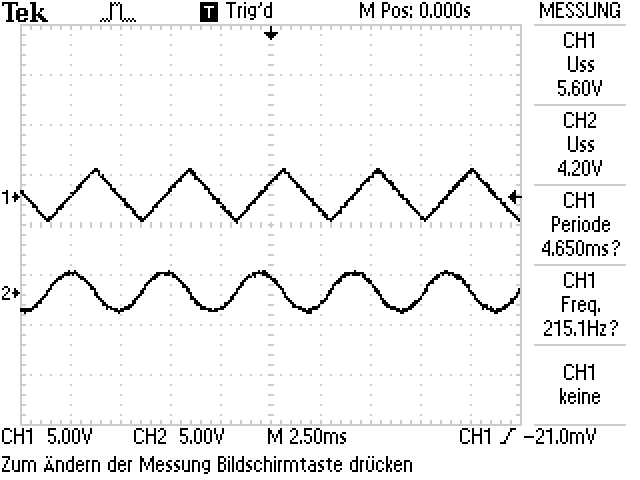
\includegraphics[width=\textwidth]{data_of_others_cuz_ours_suck/int/int_dreieck.JPG}
        \caption{Oszillographische Darstellung einer integrierten Dreieckspannung.
        Die integrierte Dreieckspannung ist auf Channel 2 dargestellt und zeigt einen Sinus.\cite{int_picture}}
        \label{fig:int_drei}
    \end{subfigure}
       \caption{Ein- und Ausgangssignale eines invertierenden Integrators. Channel 1 zeigt
       das Eingangssignal. Channel 2 zeigt das integrierte Signal.
       Die zugrunde liegende 
       Schaltung ist die des invertierenden Integrators \autoref{fig:UmkehrInt}.}
       \label{fig:int}
\end{figure}
\FloatBarrier


\subsection{Der invertierende Differenzierer \cite{int_data}, \cite{int_picture}}
Analog zu dem invertierende Integrator lassen sich die gleichen Betrachtungen 
für einen invertierenden Differenzierer anstellen.
Der Plot, welcher sich durch die Messwerte \autoref{tab:differenzierer} ergibt, ist in
\autoref{fig:differenzierer} zu sehen.
Anhand des Verlaufs der linearen Regression lässt sich feststellen, dass die Ausgangsspannung
im Bereich von 100\,Hz bis ca. 4000\,Hz proportional zu der Frequenz der Eingangsspannung ist.
Dies stimmt mit den Erwartungen nach \autoref{eq:Diff_Kosinus} überein.

Wird die Frequenz der Eingangsspannung weiter erhöht, beginnt die Ausgangsspannung
wieder zu sinken.
Dies ist genau der umgekehrte experimentelle Befund, welcher beim invertierenden Integrator
ebenfalls aufgetreten ist.
Dieser kann zum jetzigen Zeitpunkt noch nicht erklärt werden.
\begin{figure}
    \centering
    \includegraphics[width=0.7\linewidth]{build/differenzierer.pdf}
    \caption{Ausgangsspannung in Abhängigkeit der Frequenz.
    Der Plot entsteht durch die Schaltung des invertierenden Differenzierers \autoref{fig:InvDiff}, mit dem 
    Werten $R = \SI{100}{\kilo\ohm}$ und $C = \SI{22}{\nano\farad}$.
    Die dazugehörigen Messwerte stammen aus \cite{int_data}.}
    \label{fig:differenzierer}
\end{figure}
\FloatBarrier
Die Fitparameter der Geraden sind
\begin{align*}
    m_\text{theo} =  \SI{1,06 \pm 0,01 }{\volt\per\hertz},\quad b =\SI{-3,08 \pm 0,08}{\volt}.
\end{align*}
Vergleicht man die Steigungen mit der der Theorie
\begin{align*}
    m_\text{theo} =  \SI{1,00}{\volt\per\hertz},\quad b =\SI{-2,33}{\volt}
\end{align*}
ergibt sich eine Abweichung von 6\%.


Mit Hilfe der aufgebauten Differenziererschaltung lassen sich verschiedene Eingangssignale 
differenzieren. 
Hier werden ebenfalls eine Sinus-, eine Dreiecks- und eine Rechteckspannung 
untersucht.
Die Differenziationen sind mit Hilfe eines Oszilloskops aufgezeichnet worden.
Daraus ergeben sich die Bilder in \autoref{fig:diff}.
\begin{figure}
    \centering
    \begin{subfigure}[b]{0.45\textwidth}
        \centering
        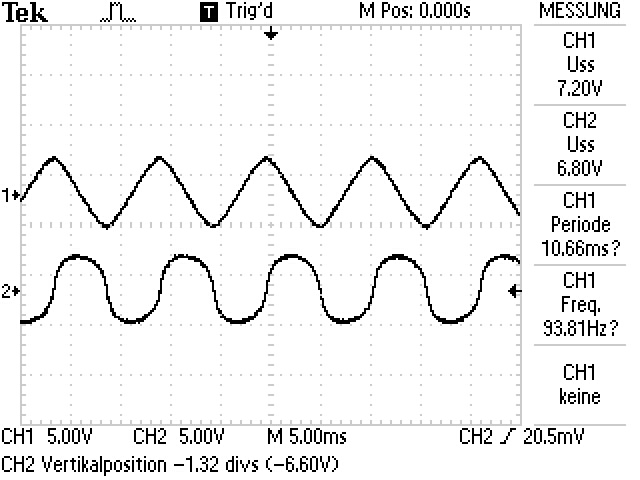
\includegraphics[width=\textwidth]{data_of_others_cuz_ours_suck/diff/diff_sin.JPG}
        \caption{Oszillographische Darstellung einer differenzierten Sinusspannung.
        Die differenzierte Sinusspannung ist auf Channel 2 dargestellt und ist ein Kosinus.\cite{int_picture}}
        \label{fig:diff_sin}
    \end{subfigure}
    \hfill
    \begin{subfigure}[b]{0.45\textwidth}
        \centering
        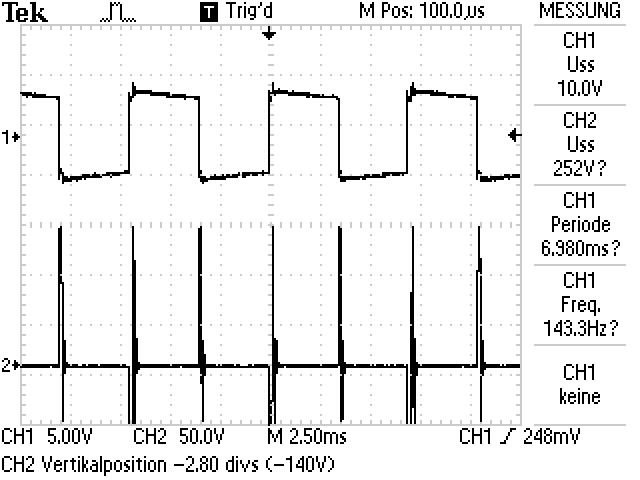
\includegraphics[width=\textwidth]{data_of_others_cuz_ours_suck/diff/diff_recht.JPG}
        \caption{Oszillographische Darstellung einer differenzierten Rechteckspannung.
        Die differenzierte Rechteckspannung ist auf Channel 2 dargestellt und sind Nadelpulse.\cite{int_picture}}
        \label{fig:diff_recht}
    \end{subfigure}
    \newline
    \newline  
    \newline
    \newline  
    \newline  
    \begin{subfigure}{0.45\textwidth}
        \centering
        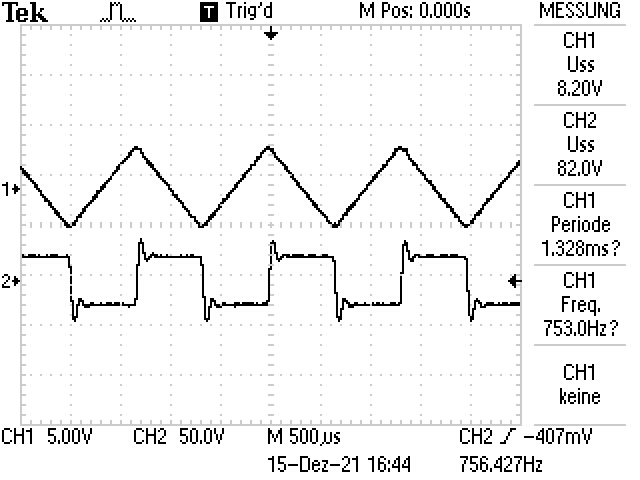
\includegraphics[width=\textwidth]{data_of_others_cuz_ours_suck/diff/diff dreieck.JPG}
        \caption{Oszillographische Darstellung einer differenzierten Dreieckspannung.
        Die differenzierte Dreieckspannung ist auf Channel 2 dargestellt und zeigt eine Rechteckspannung.\cite{int_picture}}
        \label{fig:diff_drei}
    \end{subfigure}
       \caption{Ein- und Ausgangssignale eines invertierenden Differenzierers. Channel 1 zeigt
       das Eingangssignal. Channel 2 zeigt das differenzierte Signal.}
       \label{fig:diff}
\end{figure}
\FloatBarrier

\subsection{Der nicht invertierende Schmitt-Trigger \cite{schmitt}}
In diesem Teil der Auswertung wird das Schaltverhalten eines Schmitt-Triggers \autoref{fig:Schmitt}
untersucht.
Hierbei werden für eine dreieckige Eingangsspannung die theoretischen Schaltschwellen berechnet und 
anschließend mit den im Experiment gemessenen verglichen.
Die verwendeten Bilder sind in \cite{schmitt} zu finden.

Für eine Versorgungsspannung von $U_\text{v} = \SI{\pm 15}{\volt}$ und mit
den Widerständen $R_1 = \SI{1}{\kilo\ohm}$ und $R_2 = \SI{100}{\kilo\ohm}$ ergibt sich eine 
untere und obere Schaltschwelle gemäß \autoref{eq:Schwelle} von 
\begin{align*}
    U_\text{thres, min} &=  \SI{-150}{\milli\volt},\\
    U_\text{thres, max} &=  \SI{150}{\milli\volt}.
\end{align*}
Dieses Ergebnis bedeutet, dass zu erwarten ist, dass jeweils ab $\SI{\pm150}{\milli\volt}$ 
der Schmitt-Trigger in die Hysterese schaltet.

In \autoref{fig:schmitt} ist das oszillographische Bild zu sehen.
Der orangefarbene Graph ist das Eingangssignal und der grüne das Ausgangssignal.
Erkennbar ist, dass ab einer Spannung von
\begin{equation*}
    U_\text{thres, max, gem} =  \SI{151}{\milli\volt}
\end{equation*}
der Schmitt-Trigger in die obere Aussteuergrenze läuft.
Dieser Wert wird so lange gehalten, bis die Spannung des Eingangssignals unter die 
Schwelle 
\begin{equation*}
    U_\text{thres, min, gem} =  \SI{-167}{\milli\volt}
\end{equation*}
kommt. 
Ab diesem Wert schaltet der Schmitt-Trigger in die negative Aussteuergrenze.
\begin{figure}
    \centering
    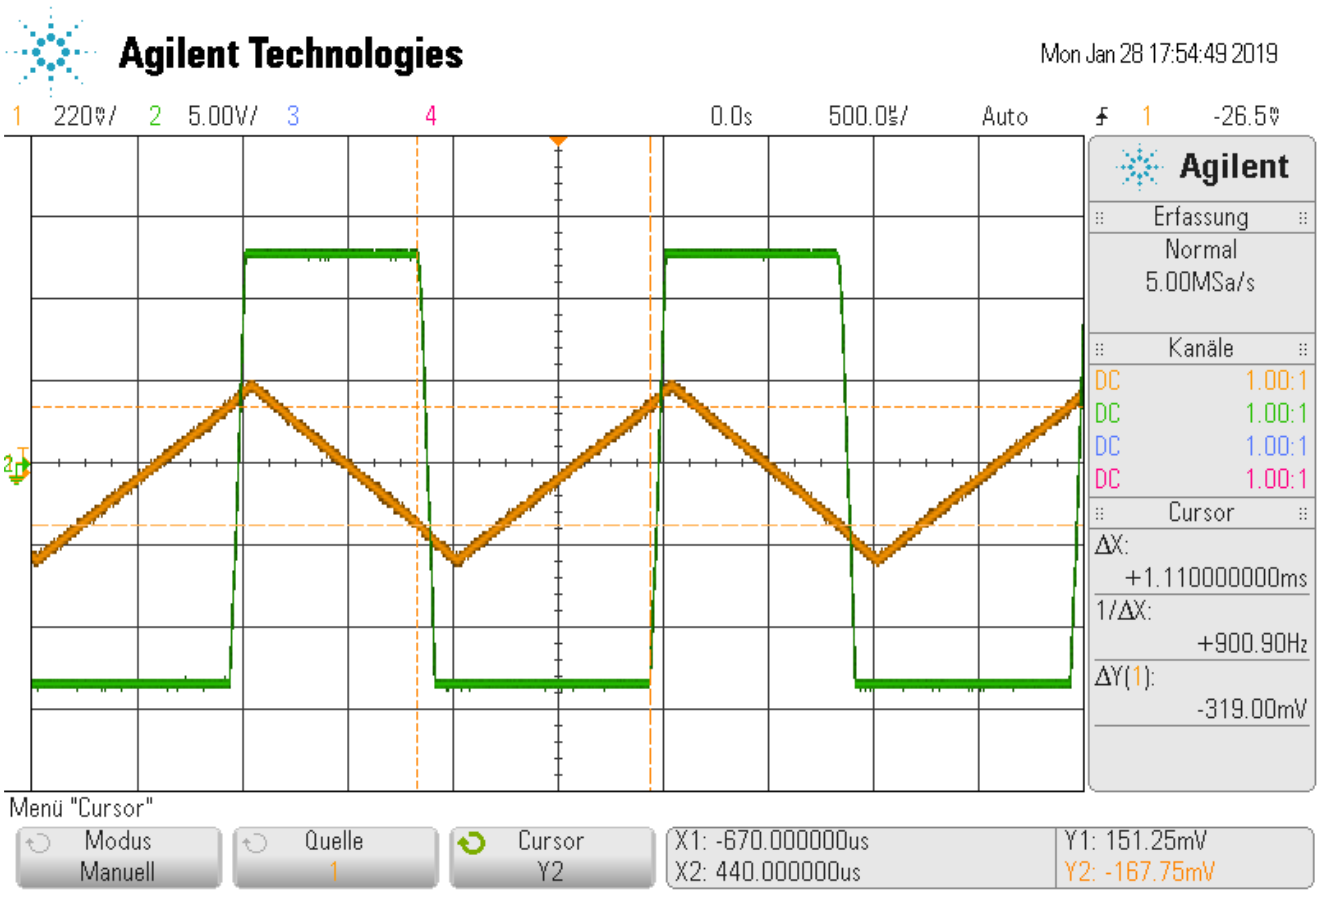
\includegraphics[width=0.7\linewidth]{data_of_others_cuz_ours_suck/schmitt/schmitt_2.png}
    \caption{Oszillographische Aufnahme des Schmitt-Triggers bei einem dreieckigen Eingangssignal. \cite{schmitt}}
    \label{fig:schmitt}
\end{figure}
\FloatBarrier
Werden die beiden gemessenen Werte verglichen, ergibt sich eine Abweichung von
0,7\% für die obere Schaltschwelle und 11\% für die untere Schaltschwelle.

\subsection{Der Signalgenerator \cite{signal}}
Wird bei einem sinusförmigen Eingangssignal hinter dem Schmitt-Trigger ein invertierender Integrator geschaltet, lässt sich 
ein Signalgenerator (vgl.\autoref{fig:Signal}) erzeugen. 
Für die im Experiment verwendeten Bauteile gilt $R_1 = \SI{1}{\kilo\ohm}$, $R_2 = \SI{100}{\kilo\ohm}$,
$R_3 = \SI{100}{\kilo\ohm}$ und $C = \SI{1}{\micro\farad}$.\cite{signal}

Da hinter dem Schmitt-Trigger ein invertierender Integrator aufgebaut ist, wird eine Dreieckspannung
als Ausgangssignal erwartet.
Das Bild, welches am Oszilloskop aufgenommen worden ist, ist in \autoref{fig:Signalgen}
zu sehen.
\begin{figure}
    \centering
    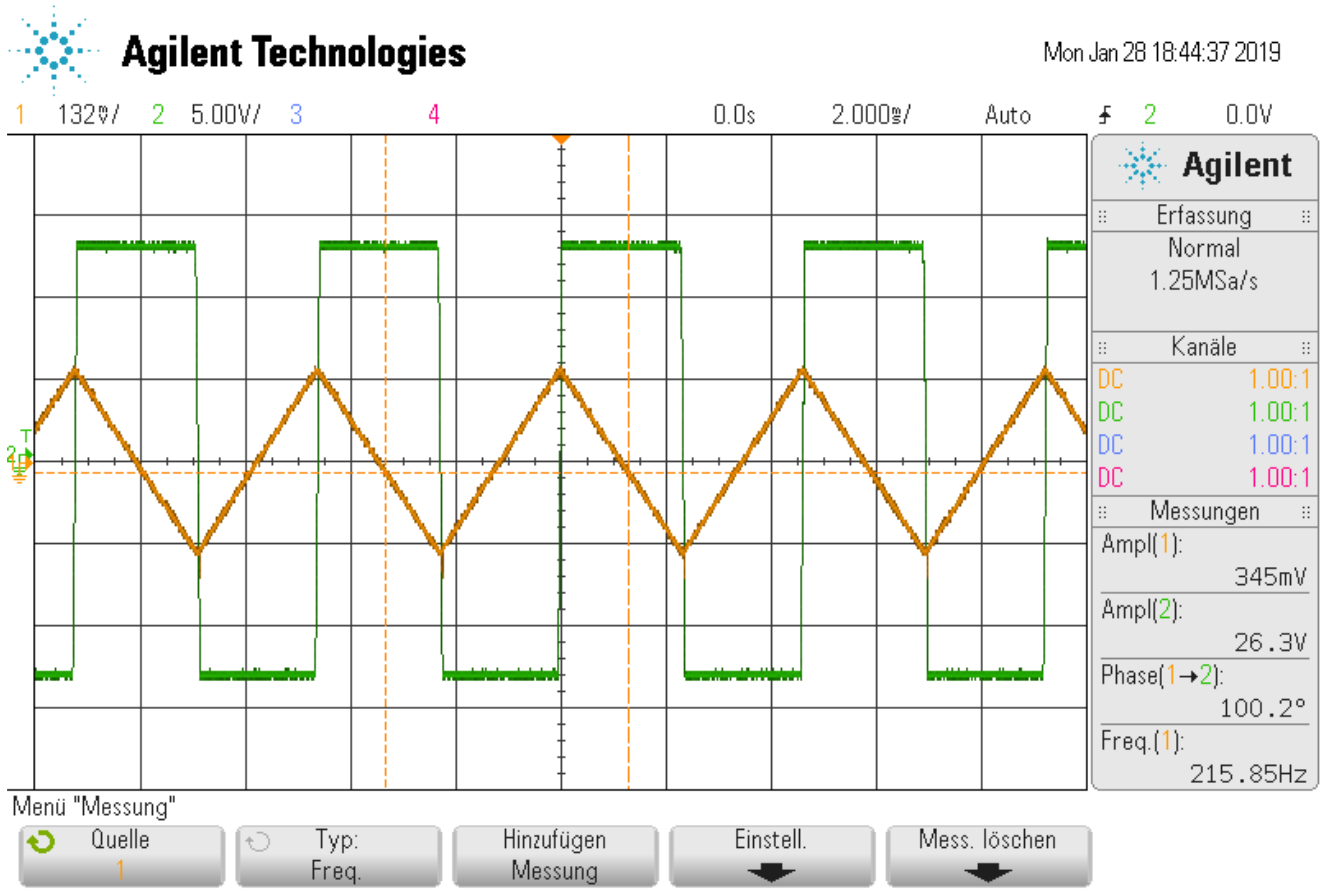
\includegraphics[width=0.7\linewidth]{data_of_others_cuz_ours_suck/Signal/Bildschirmfoto vom 2022-02-11 13-19-10.png}
    \caption{Oszillographische Aufnahme des Signals nach dem Schmitt-Trigger (grün) und 
    nach dem invertierenden Integrators. Der orangefarbene Graph ist das Ausgangssignal und die erwartete
    Dreieckspannung.\cite{signal} Das Eingangssignal ist hierbei eine Sinuspannung (nicht in der Abbildung zu sehen).}
    \label{fig:Signalgen}
\end{figure}
\FloatBarrier

Die gemessene Frequenz der Ausgangsspannung beträgt $\SI{216}{\hertz}$.
Verglichen mit dem erwarteten Wert $\SI{250}{\hertz}$, welcher sich nach \autoref{eq:Frequenz}
%\begin{equation}
%    f_\text{Dreieck} =  \frac{R_2}{4 C R_1 R_3} = \SI{250}{\hertz}
%\end{equation}
berechnet, ergibt sich eine Abweichung von 14\%.

%
%\begin{equation}\label{eq:xxx}    
%    \begin{split}
%        \lambda &= \SI{855}{\angstrom}\\
%        \delta_\text{ps} &= 0,6\cdot 10^{-6}\\
%        \delta_\text{si}&= 6,8\cdot 10^{-6} \\
%        n_\text{luft} &= 1 \\
%        n_\text{ps} &= 1 - \delta_\text{ps} \\
%        n_\text{si} &= 1 - \delta_\text{ps} 
%    \end{split}
%\end{equation}